% !TeX root = ../main.tex
% -*- coding: utf-8 -*-

\chapter{绪论}
\label{ch1}

\section{课题背景}
1946年,世界上第一台电子计算机ENIAC在美国诞生,随后的短短30年间,电子计算机的发展便经历了“电子管”、“晶体管”、“集成电路”、“大规模集成电路”四代变革,计算机体积在不断缩小的同时计算能力却提高了6个数量级。尤其是集成技术的发展,使得一小块半导体芯片上可以容纳上百万个晶体管,并且这个数量随着产品的更新迭代还在逐年增长。正如著名的摩尔定律所指出的:集成电路上可以容纳的晶体管数目在大约每经过18个月便会增加一倍\ChangeNotation。这一通过经验总结下来的定律又相当精准地预测了之后40年计算机性能的发展速度,但是随着晶体管密度的不断提高,元器件尺寸也在不断缩小,当晶体管尺寸小到接近原子尺寸时芯片性能将难以提升。2020年,台积电宣布其5纳米工艺制程芯片已进入批量生产,并且3纳米工艺也将在2021年面世。可以预见,在不久的未来摩尔定律将完全失效,经典计算机的性能也将遇到瓶颈。

为了延续甚至超越摩尔定律的辉煌,人们需要一种在底层原理上不同于经典计算机的设计,近些年来经过科研人员的不断探索,量子计算机被认为是一种能达成这一目标的途径。早在1982年,诺贝尔物理学奖得主 Richard Feynman 就提出了量子计算机的构想:既然物理世界是用量子力学的语言描述的,那么就应该用遵从量子力学原理的计算机来模拟真实世界\cite{feynman1982quantum}。1985年,牛津大学的 David Deutsch 指出可以利用相干叠加原理实现通用量子计算。1994年, Peter Shor 证明了运行于量子计算机中的算法可以实现对大数质因子的快速分解,这一算法被认为可以轻易摧毁现有的公钥加密系统并且是经典计算机所无法企及的。1998年,美国洛斯阿拉莫斯国家实验室与麻省理工、加州伯克利大学合作造出了第一台基于有机分子的2比特量子计算机并验证了量子计算的一些基本原理\ChangeNotation\cite{PhysRevLett.80.3408}。此后的十几年间,多种不同的量子计算机制造方案被提出并得到了实现,包括离子阱、量子点、超导量子比特等。但这些技术都面临着有效量子比特无法轻易做大的问题,其中主要的困难在于量子叠加态是十分脆弱的,极易因环境而发生退相干,因此必须在极短的相干时间内完成量子信息的存储、传输和处理,这就要求量子比特与操控它的光场间的耦合远大于各自的耗散,即实现所谓的强耦合\ChangeNotation\cite{PhysRevApplied.2.054002Tobar}。2001年,段路明等人提出使用原子系综(atomic ensembles)可以实现正比于粒子数平方根的强耦合\ChangeNotation,并设计了用于长程量子中继器和寄存器的方案\ChangeNotation\cite{Duan2001}。随后,超冷原子系综与光学腔间的强耦合被实验所证实。2009年,Imamo\u{g}lu 指出此前的耦合系统都是光与物质间通过电偶极相互作用来发生耦合的体系,即处于腔量子电动力学(Cavity QED)的框架下,而光与自旋粒子系综(spin ensembles)间的磁偶极相互作用能够更轻易的提高耦合率\ChangeNotation\cite{PhysRevLett.102.083602Imamoifmmode}。这一研究为人们打开了新的思路,实验上很快就出现了大量的尝试与探究。在一些自旋粒子系综体系中如超冷原子云、掺杂离子晶体、金刚石氮空位色心中均成功实现了与微波甚至超导量子比特的耦合\ChangeNotation\cite{PhysRevLett.103.043603,PhysRevLett.105.140501,PhysRevLett.105.140502}。2010年,Soykal和Flatt\'e在理论上预言了可以使用微型铁磁球中的自旋粒子集合(collection of spins)来与微波场实现强耦合\ChangeNotation\cite{PhysRevLett.104.077202Soykal}。自此之后,腔磁振子系统便开始吸引到越来越多研究者们的关注。由于此前腔量子电动力学的许多想法都可以类比过来,毫无疑问这一系统也为人们提供了用来研究强耦合QED的崭新平台,就如同离子阱、量子点和超导量子比特这些平台一样。

\section{量子关联}
量子关联是量子力学区别于经典力学的一种独有特性。早在1935年,Einstein与Podolsky,Rosen所发表的阐述EPR佯谬的文章中就展示了这种特性,随后Bell和Borm所做的验证量子关联的工作更是成为了量子信息处理领域的基石。Einstein和Bell所论述的量子关联其实是后来被称为量子纠缠的量子特性,而在量子光学领域还有另外一种量子关联,那就是包含统计意味的量子关联(相干)函数\ChangeNotation\cite{gerry2005introductory}。

自1905年Einstein提出光量子概念后的很长一段时间,大量物理光学的实验现象依旧只依赖Maxwell方程组就能描述,人们找不出经典物理与量子物理的区别。虽然一直有人在尝试从基本的光学干涉上寻找独特的量子机理,但是直到1956年,R. Hanbury Brown和R. Q. Twiss才第一次在实验上给出量子力学描述的强度干涉理解。HBT实验用两个探测器研究了入射光的强度关联,也就是二阶关联(相干)函数,并且证明了热光子的聚束行为。当时有许多物理学家意识到光子的聚束效应可以从统计的视角去理解,随后很快就有光子计数实验证明了热光子数的超泊松分布。二十世纪六十年代初,第一台激光器的诞生标志了现代光学的到来。借助激光源提供的大量相干光子,可以轻易地将一个体系从热平衡激励到高激发态。也就是在1963年的时候,R. J. Glauber提出了他的光学相干性理论。Glauber在理论中分辨出了热光子关联以及激光中相干光子关联的不同,并预言了光子的反聚束效应。反聚束的光子表现出亚泊松分布,经典理论在这里会给出负概率的矛盾。1975年,H. J. Carmichel和D. F. Walls预测了二能级原子共振荧光中光子的反聚束行为并在随后的一年中得到了实验的证实,这也是人们第一次在实验上观测到量子光学非经典效应\cite{walls2007quantum}。到了二十世纪八十年代,激光泵浦过程中的噪声限制着它的应用,而压制噪声后的激光需要表现出亚泊松的统计分布,Y. Yamamoto第一次在实验室中造出了这种半导体激光源。随后,借助参量下转换中的非线性过程单光子源也被成功造出。这些具有量子关联的新型光源具有高度的非经典性,并且已经在量子计算和量子通信等领域实现了应用。

\section{开放量子系统简介}
由于量子计算机需要不断的对信息进行读取和操作,所以用来实现量子计算机的体系都不可避免地要和环境发生相互作用,而这些系统都可以被称作为开放量子系统。早在量子光学这门学科诞生以前,就有人使用量子电动力学(QED)的方法去描述环境中原子的自发辐射,后来激光源的诞生使得人们可以从非相干的环境中激发出相干信号,而激光源本身也是一个开放量子系统。除了光源以外,还有一类重要的开放量子系统,那就是腔量子电动力学体系。腔量子电动力学可以追溯到1946年,E. M. Purcell指出原子的自发辐射会因为与有限微腔中束缚电磁场的耦合而得到增强,这一后来被称为Purcell效应的现象于1954年在核磁共振系统中得到了证实并且随后被发现广泛存在于光与物质相互作用的体系之中。正如Purcell效应所说的那样,腔量子电动力学处理的是限制在反射壁所包围的腔里的原子与腔中光场之间的相互作用,由于光在腔壁之间的来回反射,大大增加了原子与光之间的相互作用时间,使得单个光子的能量密度就足以把原子体系激发到远离热平衡的态。而在这样的情况下,经典量子电动力学的处理少量光子散射的微扰计算就不再适用,必须借助别的方法处理这样的开放量子系统。

量子光学领域中的计算涉及到许多理论方法,实际研究中可能会用到薛定谔方程、海森堡运动方程,又或者微扰理论甚至是量子场论中的工具。但是在处理开放量子系统时通常来说只有两种方法,一种是基于海森堡绘景的量子朗之万方程,另一种是基于薛定谔绘景的主方程\cite{carmichael1999statistical}。这两种方法非常接近,在选取的时候要根据实际问题的难易程度来定。通常情况下,量子朗之万方程对于非线性问题并不能得到很好的解,而这时候使用主方程却能够给出合理的解析解\cite{carmichael1999statistical}。主方程方法在过去几十年间的发展依赖于Glauber的相干性理论,其中最主要的是需要用到Glauber与Sudarshan提出的对角化相干态表象。在基于这一表象的相空间中允许把算符形式的主方程重写为经典的Fokker-Planck方程,因此在许多系统中都得到了广泛的应用。

\section{腔磁振子系统的研究现状}
腔磁振子系统指的是磁性材料中的元激发,也就是磁振子与微腔中束缚电磁场相互作用的系统。在Soykal和Flatt\'e提出使用铁磁球中的自旋粒子集合来与微波场通过Zeeman相互作用实现强耦合的方案后,人们就开始寻找合适的铁磁材料并用微波腔进行实验验证。在已有的铁磁材料之中,钇铁石榴石铁氧体(YIG,$\mathrm{Y_3Fe_5O_{12}}$)的特性格外卓越。YIG有着相当高的自旋密度$\rho=2\times10^{22}~\mathrm{cm}^{-3}$,以及非常低的Gilbert耗散率$\alpha \sim 10^{-4}$。实验上通常使用YIG的Kittel模式来实现强耦合,为达成这一点需要使用毫米尺度的小球或者薄膜并把它置于微波腔中磁场的波峰处以分离其他模式的影响。在这样装置中,YIG球的Kittel模式能够与微波腔发生共振,其铁磁共振固有线宽$\kappa_m/2\pi=\alpha \omega_m/2\pi$在1MHz量级,而选择合适的腔和YIG形状后耦合率可以很容易地达到几十上百MHz,满足强耦合的条件。当系统产生强耦合时,微波腔中的光子和磁振子会变得不再区分彼此并共同组成被称为polariton的准粒子,在观测上光场的输出强度谱就会表现出反交错(anticrossing)的现象。早期的实验中,许多研究组使用不同的微波腔和YIG都各自独立地实现了腔磁振子系统的强耦合。2013年,H. Huebl等人率先在 $50$ mK的温度中使用长条形掺镓YIG样品与超导共面波导谐振器耦合,并在实验中观测到了透射谱的反交错现象\cite{PhysRevLett.111.127003Huebl},这标志着强耦合腔磁振子系统的首次实现。2014年, M. E. Tobar 与 Y. Nakamura 两个组也各自独立地在低温(mK)下完成了微波腔与YIG球之间的强耦合实验,其中Tobar组使用的是重入式谐振腔\cite{PhysRevApplied.2.054002Tobar},而Nakamura组使用的则是定制的无氧铜三维腔\cite{PhysRevLett.113.083603Nakamura}。同年, H. Tang 课题组完成了腔磁振子系统研究中的又一个标志性成果,他们将强耦合做到了室温并且使用多组不同的微波腔与YIG球实现了多套耦合参数体制,观测到了腔磁振子系统的反交错现象、磁诱导透明(MIT,magnetically induced transparency)、Purcell效应以及超强耦合现象\cite{PhysRevLett.113.156401Tang}。2015年, C.-M. Hu 课题组使用自旋电子学的技术在LCR电路中模拟腔磁振子强耦合实验,并对YIG薄膜中的磁振子模式首次进行了间接的电学测量\cite{PhysRevLett.114.227201Hu}。在这些实现腔磁振子系统强耦合的代表性工作中所使用的装置以及主要
%随后在各种平台上构建的腔磁振子系统如雨后春笋般涌现
\begin{center}
	\tablecaption{腔磁振系统实现强耦合的实验以及主要参数}\label{ExperimentsTable}
	\begin{tabular}{ccc}
		\toprule
		实验装置及现象 & 强耦合参数 & 参考文献 \\
		\midrule
		\begin{minipage}[m]{.3\textwidth}\centering\vspace*{5pt}
			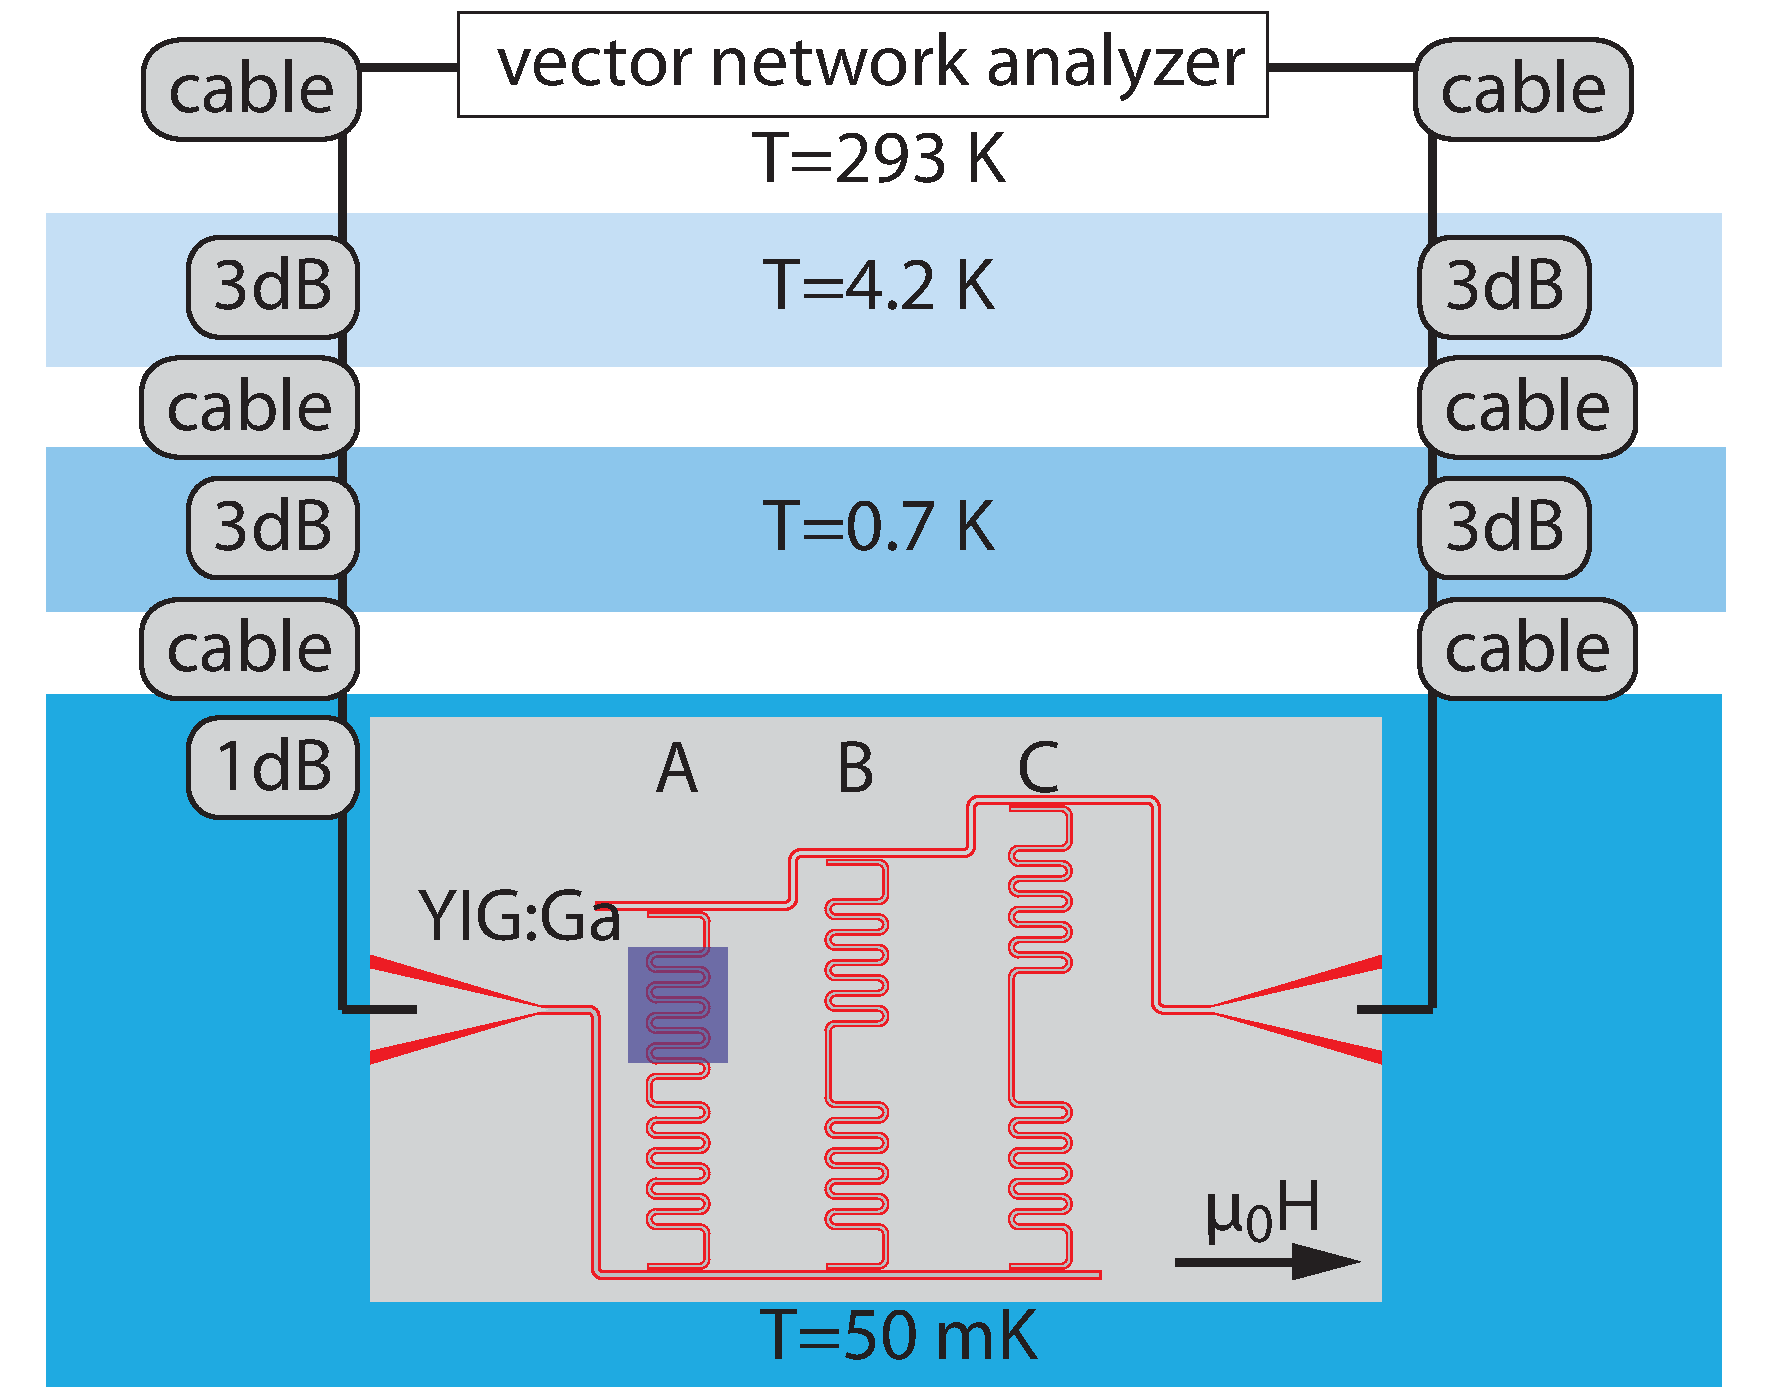
\includegraphics[width=.45\textwidth]{Table1_1}
			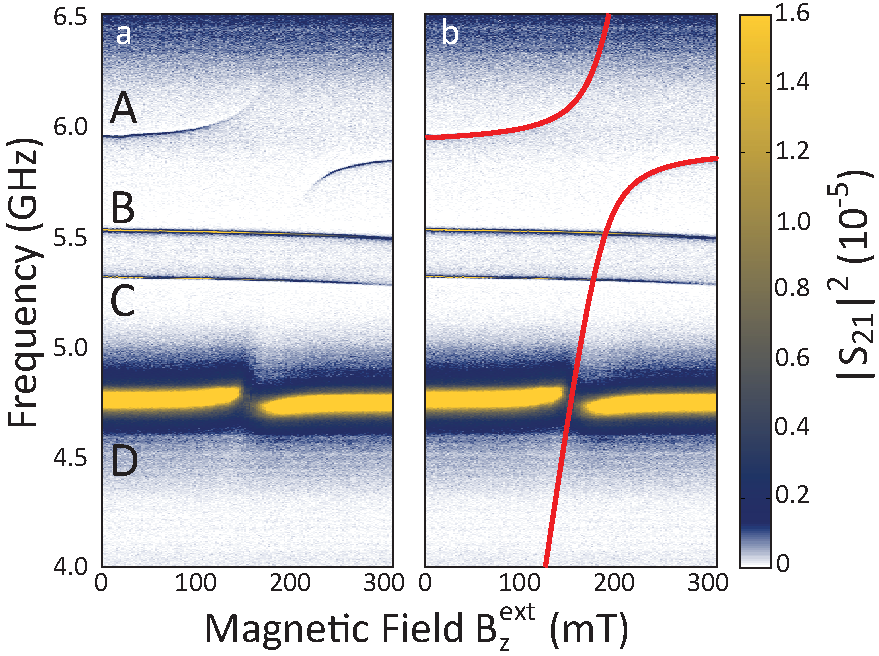
\includegraphics[width=.47\textwidth]{Table1_2}\vspace*{5pt}
		\end{minipage} &
		\begin{minipage}[m]{.5\textwidth}
			\begin{itemize}
				\item 耦合率:$g/2\pi=450$ MHz
				\item 微腔耗散率: $\kappa_c /2\pi=3$ MHz
				\item 磁振子耗散率: $\kappa_m /2\pi=50$ MHz
			\end{itemize}
		\end{minipage} &
		\parencite{PhysRevLett.111.127003Huebl} \\
		\hline
		\begin{minipage}[m]{.3\textwidth}\centering\vspace*{5pt}
			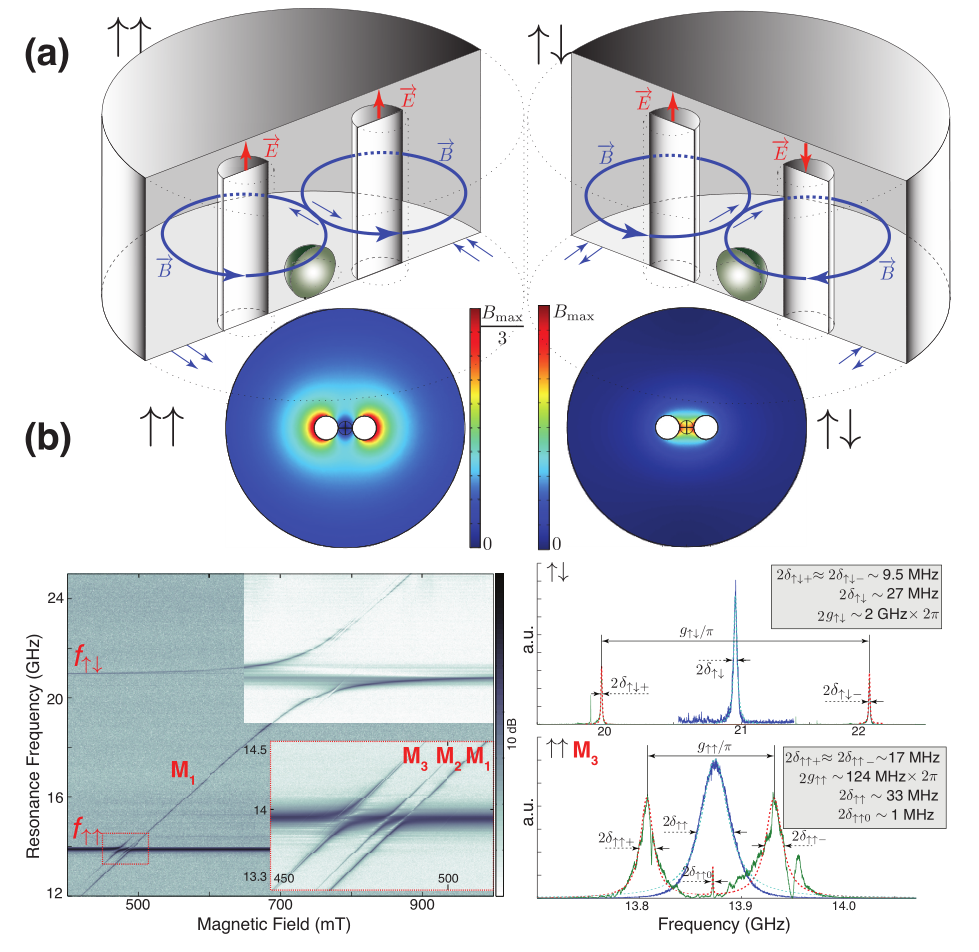
\includegraphics[width=.7\textwidth]{Table1_3}
			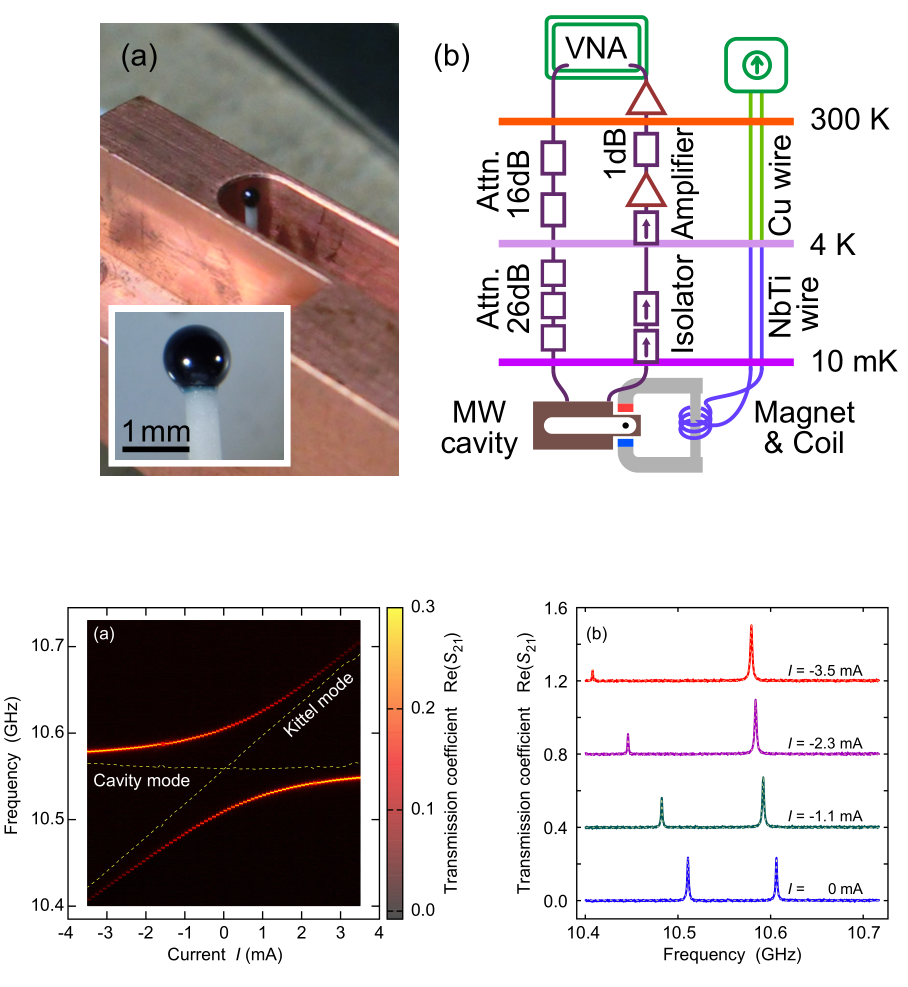
\includegraphics[width=.7\textwidth]{Table1_4}\vspace*{5pt}
		\end{minipage} &
		\begin{minipage}[m]{.5\textwidth}
			\begin{itemize}
				\item 耦合率:$g/2\pi=2$ GHz
				\item 微腔耗散率: $\kappa_c /2\pi=27$ MHz
				\item 磁振子耗散率: $\kappa_m /2\pi=1.1$ MHz
			\end{itemize}
		\end{minipage} &
		\parencite{PhysRevApplied.2.054002Tobar} \\
		\hline
		\begin{minipage}[m]{.3\textwidth}\centering\vspace*{5pt}
			\quad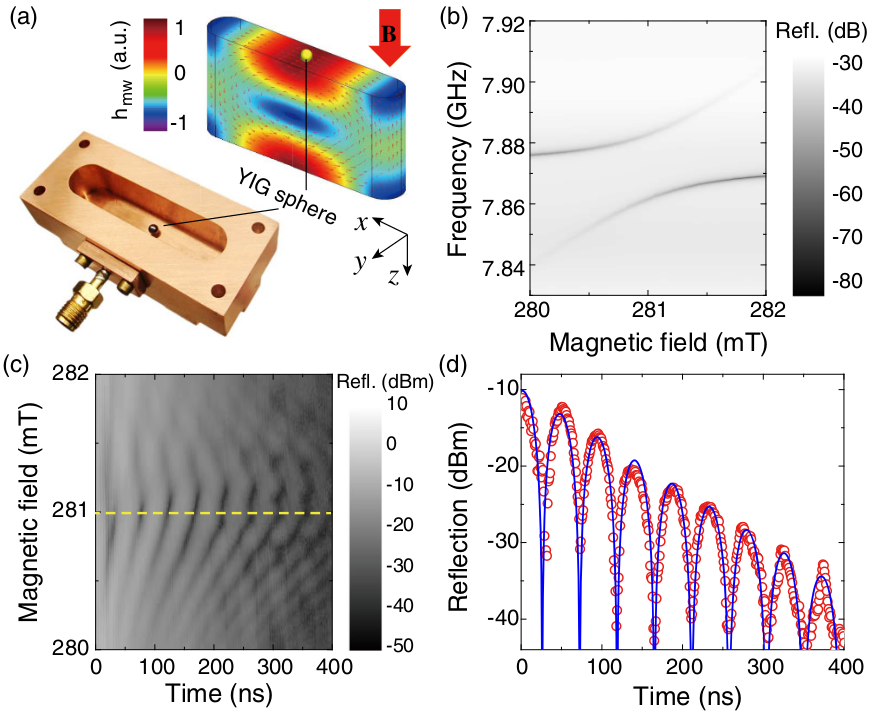
\includegraphics[width=.7\textwidth]{Table1_5}
			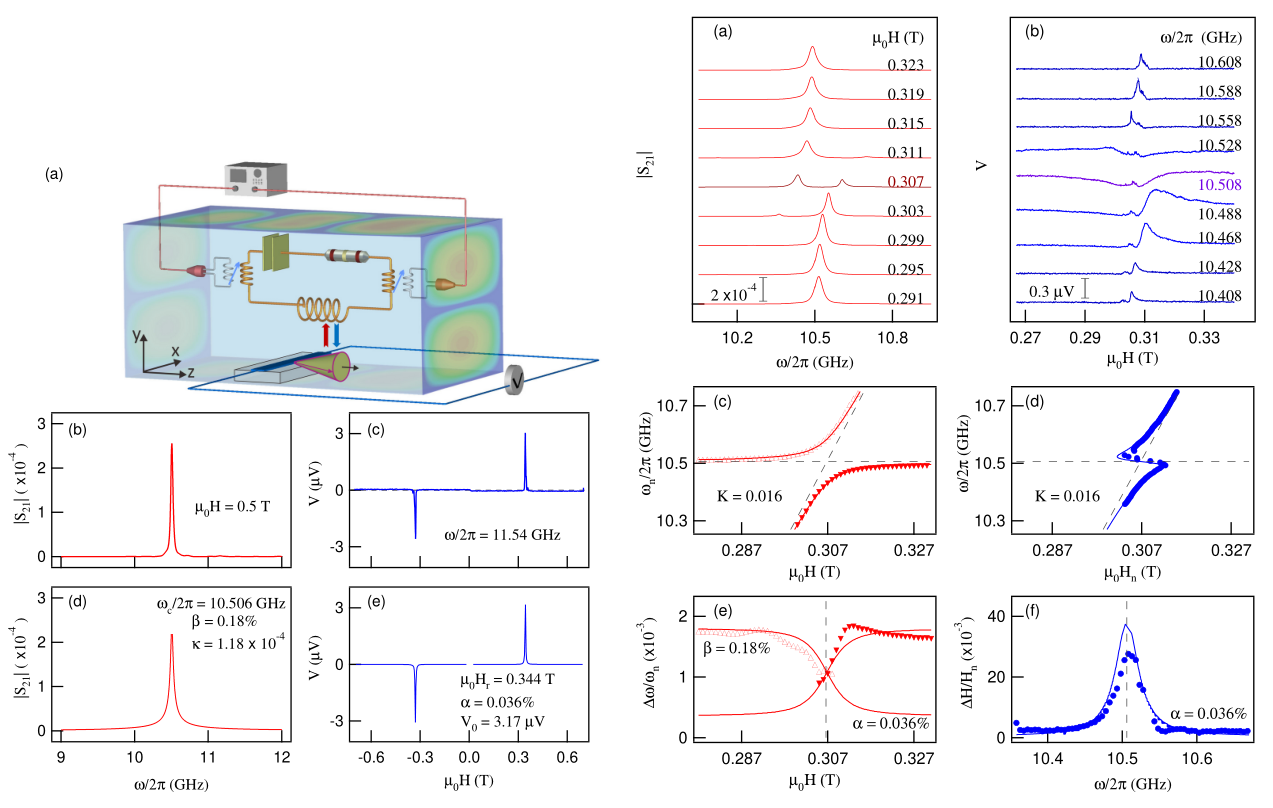
\includegraphics[width=.7\textwidth]{Table1_6}\vspace*{5pt}
		\end{minipage} &
		\begin{minipage}[m]{.5\textwidth}
			\begin{itemize}
				\item 耦合率:$g/2\pi=47$ MHz
				\item 微腔耗散率: $\kappa_c /2\pi=2.7$ MHz
				\item 磁振子耗散率: $\kappa_m /2\pi=1.1$ MHz
			\end{itemize}
		\end{minipage} &
		\parencite{PhysRevLett.113.083603Nakamura} \\
		\hline
		\begin{minipage}[m]{.3\textwidth}\centering\vspace*{5pt}
			\includegraphics[width=\textwidth]{Table1_7}\vspace*{5pt}
		\end{minipage} &
		\begin{minipage}[m]{.5\textwidth}
			\begin{itemize}
				\item 耦合率:$g/2\pi=10.8$ MHz
				\item 微腔耗散率: $\kappa_c /2\pi=1.35$ MHz
				\item 磁振子耗散率: $\kappa_m /2\pi=1.06$ MHz
			\end{itemize}
		\end{minipage} &
		\parencite{PhysRevLett.113.156401Tang} \\
		\hline
		\begin{minipage}[m]{.3\textwidth}\centering\vspace*{5pt}
			\includegraphics[width=.45\textwidth]{Table1_8}
			\includegraphics[width=.47\textwidth]{Table1_9}\vspace*{5pt}
		\end{minipage} &
		\begin{minipage}[m]{.5\textwidth}
			\begin{itemize}
				\item 耦合率:$g/2\pi=168$ MHz
				\item 微腔耗散率: $\kappa_c /2\pi=18.9$ MHz
				\item 磁振子耗散率: $\kappa_m /2\pi=3.8$ MHz
			\end{itemize}
		\end{minipage} &
		\parencite{PhysRevLett.114.227201Hu} \\
		\bottomrule
	\end{tabular}
\end{center}
实验现象见表\ref{ExperimentsTable}。在实现微波腔与磁振子的强耦合之后,这个方向的研究还远没有停歇,人们又进一步地朝非线性光学、混合量子系统以及测量应用方面迈进。2016年,浙江大学的游建强等人在实验上做出了磁振子的Kerr非线性效应\cite{PhysRevB.94.224410You},为磁振子更复杂的动力学研究打开了大门。此后, H. Tang 小组又将腔磁振子系统和YIG球中的声子模式耦合\cite{10.1126/sciadv.1501286Tang},并借用腔光力学的特征开启了腔磁振子力学系统的研究,而 Y. Nakamura 小组则将腔磁振子系统与超导量子比特进行耦合借以得到了磁振子的数态\cite{10.1126/sciadv.1603150Nakamura},二者都朝混合量子系统的方向实现了突破。另一方面, M. E. Tobar 小组进一步地将腔与YIG间的耦合率提升到7GHz,实现了所谓的超强耦合\cite{PhysRevB.93.144420Tobar}。2020年, G. Ruoso 小组利用腔磁振子系统的超强耦合实现了磁场的超高精度测量\cite{10.1063/5.0024369Ruoso},为腔磁振子系统的应用奠定了基础。

\begin{figure}[htbp]
	\centering
	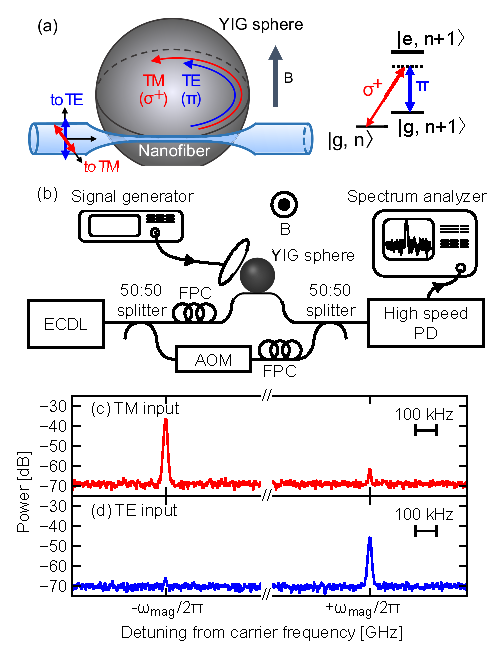
\includegraphics[width=0.33\textwidth,clip]{1_1}
	\caption{回音壁模式微腔与YIG球的耦合实验\cite{PhysRevLett.116.223601Nakamura}} 
	\label{FigOpticalCavity}
\end{figure}
虽然YIG的铁磁共振频率在GHz,但是依旧可以和光学微腔中的近红外THz波产生耦合,只不过此时的YIG与光波磁场分量间的Zeeman相互作用会被极大地压制,耦合的主要原因在于光子在磁振子中发生的布里渊弹性散射过程。由磁振子导致的布里渊光散射早有人研究,但是长久以来通信技术中使用的磁性材料都被认为是对光频透明的,原因在于耦合过于微弱。伴随着回音壁模式光学微腔的发展,实验中逐渐能够取得较为增强的耦合,一个典型的回音壁腔与YIG球耦合的实验装置如图\ref{FigOpticalCavity}所示。虽然目前为止的实验都依旧尚未实现光学腔与磁振子之间的强耦合,但是人们一直在想办法增强光学腔与磁振子之间的相互作用,提出了一系列改进实验的设想\cite{Pantazopoulos_2018,PhysRevB.98.241406Graf,PhysRevResearch.3.013277Graf}。另一方面,由于微波腔与磁振子强耦合的实现,更是促进了人们对在光频区调控磁振子并与微波区进行转换的研究热情。

这些年来腔磁振子系统在实验上的研究如火如荼取得进展的同时,对这个系统理论上的探讨也在同步进行着。Soykal和Flatt\'e对于强耦合的预言建立在Rabi模型上,Huebl的实验中使用了这一描述。Nakamura与Tang的实验中采用的是玻色子耦合的Hopfield模型,并分别用量子朗之万方程结合输入--输出理论计算了系统稳态时的透射谱和反射谱。而Hu组的理论模型则基于更经典的电磁学框架,以描述LCR电路中的电流。在非线性实验中,游建强使用玻色子算符给出了Kerr效应耦合的哈密顿量,并且也使用了量子朗之万方程来计算系统的稳态透射谱。除此之外,还有很多吸引人的对腔磁振子系统中新奇量子现象的研究。对于微波腔耦合,2017年,C.-M. Hu课题组在实验和理论上证明了腔磁振子力学系统中的拓扑性质\cite{PhysRevB.95.214411Hu},在随后的一年又提出了腔磁振子系统中源于耗散耦合的非厄米哈密顿量\cite{PhysRevLett.121.137203Hu};2018年,G. S. Agarwal等人探究了腔磁振子力学系统中的两组分以及三组分量子纠缠度并很快提出了借助Kerr非线性效应实现同一个腔中两个YIG间量子纠缠的方案\cite{PhysRevLett.121.203601Agarwal};2019年,华中科技大学的熊豪与吴颖合作研究了由磁振子的Kerr非线性所产生的非互易性\cite{PhysRevApplied.12.034001Xiong}。而在光学腔耦合领域,2018年,S. Sharma等人指出借助布里渊散射可以实现光学腔中磁振子的冷却\cite{PhysRevLett.121.087205Sharma};2019年,Bittencourt等人提出了一种实现磁振子Fock态的协议\cite{PhysRevA.100.013810Bittencourt}。这些新颖的量子效应正驱使着越来越多的人们加入到腔磁振子系统的研究当中。

\section{本文的主要内容与结构安排}
以往对腔磁振子系统的理论研究采用的多是半经典理论或者是结合量子朗之万方程的输入--输出理论,无法直接了解到系统中量子态的性质。因此我们的主要研究内容是使用量子光学中的主方程方法来探究腔磁振子系统中包括量子关联在内的一些量子性质。

在第二章中我们会首先介绍并导出我们所研究的腔磁振子系统哈密顿量,包括光子部分以及光与磁振子的耦合部分。接下来会详细推导我们所使用的主方程方法,借助密度算符以及相互作用表象,在Born--Markov近似下给出腔磁振子系统的主方程。然后通过相干态表象,进一步地将主方程变换为Fokker-Planck方程,随之得到数学上等价的随机微分方程。最后我们会简单介绍随机微分方程数值模拟的算法。

在第三章中我们会探究腔磁振子系统的稳态谱。首先通过假设稳态的形式,我们可以得到共振条件下平均粒子数与二阶关联函数的解析解。接着我们会基于 H. Tang 课题组实验上的参数分别计算强耦合、MIT以及Purcell效应三种不同情景下的稳态谱,并用解析解做出理解。

在第四章中我们会使用随机微分方程模拟的方法来研究腔磁振子系统的动力学演化行为。首先在连续驱动的情况下,我们会探究系统是如何从给定的初态演化到稳态的,并将模拟得到的稳态值与第三章的结果互相验证。然后我们会在实验可达到的条件下模拟脉冲激励下的时间演化,观察并分析强耦合、MIT以及Purcell三种参数下的动力学行为。
